\documentclass[aspectratio=169]{beamer}

% Theme & Color Settings
\usetheme{Madrid}
\usecolortheme{seahorse}

\usepackage{booktabs}
\usepackage{hyperref}
\usepackage{listings}
\usepackage{xcolor}
\usepackage{tikz}
\usetikzlibrary{arrows.meta, positioning, shapes.geometric}

\definecolor{codebg}{rgb}{0.95,0.95,0.95}
\definecolor{darnitblue}{rgb}{0.12,0.47,0.71}
\definecolor{alertred}{rgb}{0.84,0.15,0.16}

\lstset{
    backgroundcolor=\color{codebg},
    basicstyle=\ttfamily\scriptsize,
    breaklines=true,
    frame=single,
    rulecolor=\color{gray!30}
}

% Presentation Metadata
\title[Darnit Reproducibility Evaluation]{Reproducibility in Darnit: Experiments \& Upstream Issues}
\subtitle{Testing runtime non-determinism, identifying blind spots, and 7 upstream fixes}
\author[Jaydeep]{Jaydeep}
\institute[Darnit Community]{Darnit Weekly Community Sync}
\date{September 2026}

\begin{document}

% Slide 1: Title
\begin{frame}
    \titlepage
\end{frame}

% Slide 2: Agenda
\begin{frame}{Overview: What We Tested \& Issues Filed}
    \framesubtitle{Summary of engine fixes, experiment targets, and upstream roadmap alignment}
    \begin{enumerate}
        \item \textbf{Core Engine Fixes:}
        \begin{itemize}
            \item Issue \#427: CLI implementation discovery failure (tested fix ready!)
            \item Issue \#428: Output order stability in CLI (\texttt{merger.py} set iteration)
        \end{itemize}
        \item \textbf{Three Concrete Experiments:}
        \begin{itemize}
            \item Exp 1 (NumPy): Multithreaded OpenBLAS reduction divergence \& Issue \#429
            \item Exp 2 (C + ctypes): Compiler optimization flags (-ffast-math) \& Issues \#432, \#433
            \item Exp 3 (NDSS'25): Badged research artifact audit \& Issues \#430, \#431
        \end{itemize}
        \item \textbf{Upstream Roadmap Alignment:} Contributing to Tier 1 Determinism (\#418), Heuristics (\#416), and Scientific Ontology (\#393)
    \end{enumerate}
\end{frame}

% Slide 3: Universal Bug 1 (#427)
\begin{frame}{Plugin Handler Discovery in CLI}
    \framesubtitle{Core Engine Fix $\cdot$ Issue \#427}
    \begin{columns}[T]
        \begin{column}{0.48\textwidth}
            \begin{alertblock}{The Problem \& Root Cause}
                \small
                \begin{itemize}
                    \item \texttt{cmd\_audit} resolved TOML config via \texttt{darnit.frameworks}, but \textbf{never invoked \texttt{discover\_implementations()}}.
                    \item Handlers (e.g. \texttt{repro\_deps\_pinned}) were never registered into \texttt{SieveHandlerRegistry}.
                    \item \textbf{Result:} Every control warned \textit{"handler not found in registry"} and fell back to manual \texttt{WARN}.
                \end{itemize}
            \end{alertblock}
        \end{column}
        \begin{column}{0.48\textwidth}
            \begin{block}{How We Solved It}
                \small
                In \texttt{packages/darnit/src/darnit/cli.py} inside \texttt{cmd\_audit}:
                \begin{lstlisting}[language=Python]
from darnit.core.discovery import discover_implementations

# Discover & register plugin handlers
discover_implementations()
                \end{lstlisting}
                \vspace{0.1cm}
                \textbf{Current Status:} Tested and verified locally on branch. Sieve handlers now execute properly. Ready to submit PR today.
            \end{block}
        \end{column}
    \end{columns}
\end{frame}

% Slide 4: Universal Bug 2 (#428)
\begin{frame}{Deterministic Output Ordering in CLI}
    \framesubtitle{Core Engine Fix $\cdot$ Issue \#428}
    \begin{columns}[T]
        \begin{column}{0.48\textwidth}
            \begin{alertblock}{The Problem \& Root Cause}
                \small
                \begin{itemize}
                    \item Running \texttt{darnit audit --show-all} twice against unchanged repositories caused warning lines to randomly swap positions.
                    \item \textbf{Root Cause:} In \texttt{merger.py:424}:
                    \begin{lstlisting}[language=Python]
all_control_ids: set[str] = set(framework.controls.keys())
for control_id in all_control_ids:
    effective.controls[control_id] = ...
                    \end{lstlisting}
                    \item Python \texttt{set} iteration order varies with process-randomized \texttt{PYTHONHASHSEED}.
                \end{itemize}
            \end{alertblock}
        \end{column}
        \begin{column}{0.48\textwidth}
            \begin{block}{Connection to Maintainer Roadmap (\#418)}
                \small
                \begin{itemize}
                    \item Connects directly to Michael Lieberman's \textbf{\#418} (Determinism Tier 1).
                    \item \textbf{Solution:} Preserve framework control list order or sort control IDs.
                    \item With \texttt{PYTHONHASHSEED=0}, outputs were 100\% byte-for-byte identical across runs.
                \end{itemize}
            \end{block}
        \end{column}
    \end{columns}
\end{frame}

% Slide 5: Exp 1 Flow & Numerical Trap
\begin{frame}{Multithreaded NumPy BLAS Divergence}
    \framesubtitle{Experiment 1 $\cdot$ Setup \& Run}
    \centering
    \resizebox{0.95\textwidth}{!}{
    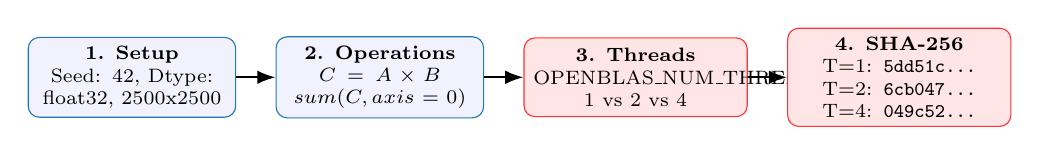
\begin{tikzpicture}[node distance=0.5cm, auto,
        block/.style={rectangle, draw=darnitblue, fill=blue!5, text width=2.4cm, text centered, rounded corners, minimum height=1cm, font=\scriptsize},
        highlight/.style={rectangle, draw=red!80, fill=red!10, text width=2.6cm, text centered, rounded corners, minimum height=1cm, font=\scriptsize},
        line/.style={draw, -Latex, thick}]
        
        \node [block] (seed) {\textbf{1. Setup}\\Seed: 42, Dtype: float32, 2500x2500};
        \node [block, right=of seed] (ops) {\textbf{2. Operations}\\$C = A \times B$\\$\text{sum}(C, \text{axis}=0)$};
        \node [highlight, right=of ops] (threads) {\textbf{3. Threads}\\OPENBLAS\_NUM\_THREADS\\1 vs 2 vs 4};
        \node [highlight, right=of threads] (hash) {\textbf{4. SHA-256}\\T=1: \texttt{5dd51c...}\\T=2: \texttt{6cb047...}\\T=4: \texttt{049c52...}};
        
        \path [line] (seed) -- (ops);
        \path [line] (ops) -- (threads);
        \path [line] (threads) -- (hash);
    \end{tikzpicture}
    }
    
    \vspace{0.3cm}
    \begin{columns}[T]
        \begin{column}{0.48\textwidth}
            \footnotesize
            \textbf{Why numbers diverged:}
            \begin{itemize}
                \item Floating-point non-associativity: $(a + b) + c \neq a + (b + c)$.
                \item Worker threads accumulate partial blocks in differing sequences.
                \item \textbf{763 of 2,500 elements (30.52\%)} differed between 1 and 2 threads.
            \end{itemize}
        \end{column}
        \begin{column}{0.48\textwidth}
            \footnotesize
            \textbf{Intra-thread repeatability verified:}
            \begin{itemize}
                \item 3 consecutive runs with fixed thread count yielded 100\% byte-identical digests.
                \item Non-determinism stems purely from runtime thread concurrency.
            \end{itemize}
        \end{column}
    \end{columns}
\end{frame}

% Slide 6: Exp 1 Darnit Results & Bug #429
\begin{frame}{Darnit Results \& Dependency Pinning}
    \framesubtitle{Experiment 1 $\cdot$ Audit Findings $\cdot$ Issue \#429}
    \begin{columns}[T]
        \begin{column}{0.48\textwidth}
            \begin{block}{Semantic Gap in Dependency Pinning}
                \small
                \begin{itemize}
                    \item Target with \texttt{uv.lock} received a green \textbf{PASS} on \texttt{RE-01.01}.
                    \item \textbf{Blind Spot:} A lockfile pins the Python package, but leaves underlying BLAS/C runtime thread scheduling unconstrained.
                    \item Software that passed all Darnit checks still suffered 30.5\% numerical divergence across machines.
                \end{itemize}
            \end{block}
        \end{column}
        \begin{column}{0.48\textwidth}
            \begin{alertblock}{Issue \#429: False Positive on requirements.txt}
                \small
                \begin{itemize}
                    \item When tested with \texttt{requirements.txt} containing strict pin \texttt{numpy==2.5.2}, Darnit returned a hard \textbf{FAIL}.
                    \item \texttt{repro\_deps\_pinned} hardcodes \texttt{requirements.txt} as a "loose manifest" without inspecting contents.
                    \item \textbf{Fix:} Inspect file lines; if all non-comment lines have exact \texttt{==} pins or hashes, do not fail outright as loose.
                \end{itemize}
            \end{alertblock}
        \end{column}
    \end{columns}
\end{frame}

% Slide 7: Exp 2 Flow & Fast-Math Trap
\begin{frame}{C Compilation \& Optimization Flags}
    \framesubtitle{Experiment 2 $\cdot$ Setup \& Run}
    \centering
    \resizebox{0.95\textwidth}{!}{
    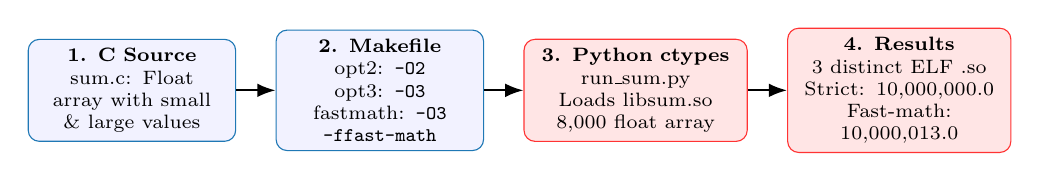
\begin{tikzpicture}[node distance=0.5cm, auto,
        block/.style={rectangle, draw=darnitblue, fill=blue!5, text width=2.4cm, text centered, rounded corners, minimum height=1cm, font=\scriptsize},
        highlight/.style={rectangle, draw=red!80, fill=red!10, text width=2.6cm, text centered, rounded corners, minimum height=1cm, font=\scriptsize},
        line/.style={draw, -Latex, thick}]
        
        \node [block] (source) {\textbf{1. C Source}\\sum.c: Float array with small \& large values};
        \node [block, right=of source] (make) {\textbf{2. Makefile}\\opt2: \texttt{-O2}\\opt3: \texttt{-O3}\\fastmath: \texttt{-O3 -ffast-math}};
        \node [highlight, right=of make] (ctypes) {\textbf{3. Python ctypes}\\run\_sum.py\\Loads libsum.so\\8,000 float array};
        \node [highlight, right=of ctypes] (bin) {\textbf{4. Results}\\3 distinct ELF .so\\Strict: 10,000,000.0\\Fast-math: 10,000,013.0};
        
        \path [line] (source) -- (make);
        \path [line] (make) -- (ctypes);
        \path [line] (ctypes) -- (bin);
    \end{tikzpicture}
    }
    
    \vspace{0.3cm}
    \begin{columns}[T]
        \begin{column}{0.48\textwidth}
            \footnotesize
            \textbf{Compiler mechanism:}
            \begin{itemize}
                \item Under \texttt{-O2} / \texttt{-O3}: Strict sequential accumulation; small terms truncated when added to large total.
                \item Under \texttt{-ffast-math}: Enables associative math; loops vectorized into SIMD lanes (\texttt{addps}), preserving small values.
            \end{itemize}
        \end{column}
        \begin{column}{0.48\textwidth}
            \footnotesize
            \textbf{Darnit audit score: 0 PASS / 0 FAIL / 5 WARN}
            \begin{itemize}
                \item Completely oblivious to native C compilation.
                \item Grepped Makefile only for \texttt{curl} and \texttt{wget}, ignoring \texttt{gcc} and \texttt{-ffast-math}.
            \end{itemize}
        \end{column}
    \end{columns}
\end{frame}

% Slide 8: Exp 2 Darnit Bugs (#432 & #433)
\begin{frame}{Compiler Flags \& Native Toolchains}
    \framesubtitle{Experiment 2 $\cdot$ Audit Findings $\cdot$ Issues \#432 \& \#433}
    \begin{columns}[T]
        \begin{column}{0.48\textwidth}
            \begin{alertblock}{Issue \#432: Compiler Flags in Makefiles}
                \small
                \begin{itemize}
                    \item \texttt{repro\_hermetic\_build} reported: \textit{"No suspicious patterns found in 1 scanned file(s)"}.
                    \item Completely missed \texttt{gcc} and flags like \texttt{-ffast-math} and \texttt{-Ofast} that alter float precision and binary reproducibility.
                    \item \textbf{Fix:} Add check for non-deterministic/unsafe compiler flags in build files.
                \end{itemize}
            \end{alertblock}
        \end{column}
        \begin{column}{0.48\textwidth}
            \begin{block}{Issue \#433: Native Toolchains Overlooked}
                \small
                \begin{itemize}
                    \item When C source code is present, Darnit still only looks for Dockerfiles or Python/Node lockfiles.
                    \item Does not inspect \texttt{CMakePresets.json}, Makefile toolchains (\texttt{CC = gcc-13}), or Conan/vcpkg.
                    \item \textbf{Fix:} Tailor manual verification guidance toward compiler and libc pinning when C source files exist.
                \end{itemize}
            \end{block}
        \end{column}
    \end{columns}
\end{frame}

% Slide 9: Exp 3 Flow (NDSS'25 Badged Artifact)
\begin{frame}{Auditing a Real Research Artifact (NDSS 2025)}
    \framesubtitle{Experiment 3 $\cdot$ Setup \& Run}
    \centering
    \resizebox{0.95\textwidth}{!}{
    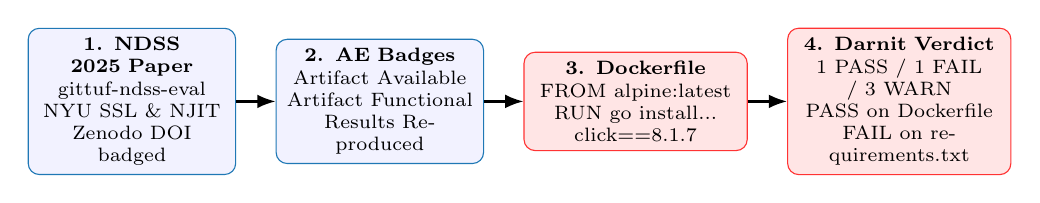
\begin{tikzpicture}[node distance=0.5cm, auto,
        block/.style={rectangle, draw=darnitblue, fill=blue!5, text width=2.4cm, text centered, rounded corners, minimum height=1cm, font=\scriptsize},
        highlight/.style={rectangle, draw=red!80, fill=red!10, text width=2.6cm, text centered, rounded corners, minimum height=1cm, font=\scriptsize},
        line/.style={draw, -Latex, thick}]
        
        \node [block] (paper) {\textbf{1. NDSS 2025 Paper}\\gittuf-ndss-eval\\NYU SSL \& NJIT\\Zenodo DOI badged};
        \node [block, right=of paper] (badges) {\textbf{2. AE Badges}\\Artifact Available\\Artifact Functional\\Results Reproduced};
        \node [highlight, right=of badges] (docker) {\textbf{3. Dockerfile}\\FROM alpine:latest\\RUN go install...\\click==8.1.7};
        \node [highlight, right=of docker] (verdict) {\textbf{4. Darnit Verdict}\\1 PASS / 1 FAIL / 3 WARN\\PASS on Dockerfile\\FAIL on requirements.txt};
        
        \path [line] (paper) -- (badges);
        \path [line] (badges) -- (docker);
        \path [line] (docker) -- (verdict);
    \end{tikzpicture}
    }
    
    \vspace{0.3cm}
    \begin{columns}[T]
        \begin{column}{0.55\textwidth}
            \footnotesize
            \textbf{Dockerfile contents inspected:}
            \begin{lstlisting}[language=bash]
FROM alpine:latest
RUN apk update && apk add git openssh go python3 py3-click
RUN go install github.com/gittuf/gittuf@v0.7.0
ADD experiment1.py ... /root/
            \end{lstlisting}
        \end{column}
        \begin{column}{0.42\textwidth}
            \footnotesize
            \textbf{Why this case matters:}
            \begin{itemize}
                \item Real-world scientific software constructed by supply-chain security researchers.
                \item Exposes the divide between academic artifact evaluation and SLSA Level 3 verification.
            \end{itemize}
        \end{column}
    \end{columns}
\end{frame}

% Slide 10: Exp 3 Darnit Bugs (#430, #431) + Ontology (#393)
\begin{frame}{Hermeticity Gaps \& Scientific Tooling}
    \framesubtitle{Experiment 3 $\cdot$ Audit Findings $\cdot$ Issues \#430 \& \#431}
    \begin{columns}[T]
        \begin{column}{0.32\textwidth}
            \begin{alertblock}{Issue \#430: Hermeticity}
                \scriptsize
                \texttt{repro\_hermetic\_build} checks pip/npm, but misses \texttt{go install} and \texttt{cargo install}.
                \texttt{RUN go install} fetched packages over the internet during build, but passed as clean!\\
                \textbf{Fix:} Add Go/Cargo/Ruby to pattern list.
            \end{alertblock}
        \end{column}
        \begin{column}{0.32\textwidth}
            \begin{alertblock}{Issue \#431: Docker PASS}
                \scriptsize
                Darnit gave confident \textbf{PASS} (0.85) simply because Dockerfile exists, ignoring unpinned floating base image (\texttt{FROM alpine:latest}) and unversioned \texttt{apk add}.\\
                \textbf{Fix:} Parse \texttt{FROM} for digest vs latest.
            \end{alertblock}
        \end{column}
        \begin{column}{0.32\textwidth}
            \begin{block}{Roadmap Alignment (\#393)}
                \scriptsize
                Academic artifacts don't publish SLSA provenance workflows. They prioritize Zenodo DOIs, execution harnesses, and container runnability.\\
                Our NDSS'25 data provides direct empirical evidence for issue \textbf{\#393}!
            \end{block}
        \end{column}
    \end{columns}
\end{frame}

% Slide 11: Summary & PR Plan
\begin{frame}{Upstream Issues \& PR Plan}
    \framesubtitle{Summary of all 7 opened issues and immediate action items}
    \small
    \begin{table}
        \centering
        \begin{tabular}{llcp{4.5cm}}
            \toprule
            \textbf{Issue} & \textbf{Category} & \textbf{Component} & \textbf{Next Action} \\
            \midrule
            \href{https://github.com/darnitdevorg/darnit/issues/427}{\textbf{\#427}} & Core Engine Bug & \texttt{cli.py} & \textbf{Submit PR today} (fix tested locally in branch) \\
            \href{https://github.com/darnitdevorg/darnit/issues/428}{\textbf{\#428}} & Core Determinism & \texttt{merger.py} & Align with Tier 1 (\#418); submit PR \\
            \href{https://github.com/darnitdevorg/darnit/issues/429}{\textbf{\#429}} & Plugin False Positive & \texttt{handlers.py} & Refine \texttt{requirements.txt} line inspection \\
            \href{https://github.com/darnitdevorg/darnit/issues/430}{\textbf{\#430}} & Hermeticity Gap & \texttt{handlers.py} & Add \texttt{go install}, \texttt{cargo install} to patterns \\
            \href{https://github.com/darnitdevorg/darnit/issues/431}{\textbf{\#431}} & Plugin False Positive & \texttt{handlers.py} & Downgrade unpinned \texttt{:latest} Dockerfiles \\
            \href{https://github.com/darnitdevorg/darnit/issues/432}{\textbf{\#432}} & Blind Spot & \texttt{handlers.py} & Check compiler flags (\texttt{-ffast-math}) in Makefiles \\
            \href{https://github.com/darnitdevorg/darnit/issues/433}{\textbf{\#433}} & Native Toolchains & \texttt{handlers.py} & Support C/C++ build manifests and toolchains \\
            \bottomrule
        \end{tabular}
    \end{table}
    \vspace{0.2cm}
    \centering
    \footnotesize Full experiment code and reports: \texttt{github.com/Jaydeep869/darnit} (branch \texttt{reproducibility-evaluation})
\end{frame}

\end{document}
